% =========================================================================
% PHẦN BÀI TẬP (TIẾP THEO MỤC 3.3) - BỐ CỤC 2 CỘT CÂN ĐỐI
% =========================================================================
\noindent
\begin{minipage}[t]{0.485\textwidth}
  \vspace{0pt}
  % Nhóm bài tập giới hạn 49 - 60
  \begin{tabularx}{\linewidth}{@{}p{0.52\linewidth}@{\hspace{4pt}}p{0.46\linewidth}@{}}
    \textbf{49.} $\lim\limits_{x \to 0} \dfrac{\sin x - \sin x \cos x}{x^2}$ & 
    \textbf{50.} $\lim\limits_{x \to 0} \dfrac{1 - \sec x}{2x}$ \\[13pt]
    \textbf{51.} $\lim\limits_{x \to 0} \dfrac{\tan 2x}{x}$ & 
    \textbf{52.} $\lim\limits_{\theta \to 0} \dfrac{\sin \theta}{\tan 7\theta}$ \\[13pt]
    \textbf{53.} $\lim\limits_{x \to 0} \dfrac{\sin 3x}{5x^3 - 4x}$ & 
    \textbf{54.} $\lim\limits_{x \to 0} \dfrac{\sin 3x \sin 5x}{x^2}$ \\[13pt]
    \textbf{55.} $\lim\limits_{\theta \to 0} \dfrac{\sin \theta}{\theta + \tan \theta}$ & 
    \textbf{56.} $\lim\limits_{x \to 0} \csc x \sin(\sin x)$ \\[13pt]
    \textbf{57.} $\lim\limits_{\theta \to 0} \dfrac{\cos \theta - 1}{2\theta^2}$ & 
    \textbf{58.} $\lim\limits_{x \to 0} \dfrac{\sin(x^2)}{x}$ \\[13pt]
    \textbf{59.} $\lim\limits_{x \to \pi/4} \dfrac{1 - \tan x}{\sin x - \cos x}$ & 
    \textbf{60.} $\lim\limits_{x \to 1} \dfrac{\sin(x - 1)}{x^2 + x - 2}$
  \end{tabularx}

  \vspace{7pt}
  {\color{stewartcyan}\rule{\linewidth}{0.6pt}}
  \vspace{3pt}

  \noindent{\color{stewartcyan}\textbf{61--62}}\quad \textsf{Tìm đạo hàm đã cho bằng cách tính một vài đạo hàm đầu tiên và quan sát quy luật xuất hiện.}

  \vspace{6pt}
  \begin{tabularx}{\linewidth}{@{}p{0.52\linewidth}@{\hspace{4pt}}p{0.46\linewidth}@{}}
    \textbf{61.} $\dfrac{d^{99}}{dx^{99}} (\sin x)$ & 
    \textbf{62.} $\dfrac{d^{35}}{dx^{35}} (x \sin x)$
  \end{tabularx}

  \vspace{4pt}
  {\color{stewartcyan}\rule{\linewidth}{0.6pt}}
  \vspace{5pt}

  \noindent\textbf{63.} Tìm các hằng số $A$ và $B$ sao cho hàm số $y = A \sin x + B \cos x$ thỏa mãn phương trình vi phân $y'' + y' - 2y = \sin x$.

  \vspace{6pt}
  \noindent\textbf{64.} (a) Tính $\lim\limits_{x \to \infty} x \sin \dfrac{1}{x}$.\\[3pt]
  \hspace*{1.6em}(b) Tính $\lim\limits_{x \to 0} x \sin \dfrac{1}{x}$.\\[3pt]
  \llap{\casicon\hspace{5pt}}(c) Minh họa các phần (a) và (b) bằng cách vẽ đồ thị $y = x \sin(1/x)$.

  \vspace{6pt}
  \noindent\textbf{65.} Lấy đạo hàm từng đồng nhất thức lượng giác để thu được một đồng nhất thức mới (hoặc quen thuộc).

  \vspace{3pt}
  \noindent
  \begin{tabularx}{\linewidth}{@{}p{0.52\linewidth}@{\hspace{4pt}}p{0.46\linewidth}@{}}
    (a) $\tan x = \dfrac{\sin x}{\cos x}$ & 
    (b) $\sec x = \dfrac{1}{\cos x}$
  \end{tabularx}\\[4pt]
  (c) $\sin x + \cos x = \dfrac{1 + \cot x}{\csc x}$
\end{minipage}%
\hfill
\begin{minipage}[t]{0.485\textwidth}
  \vspace{0pt}
  \noindent\textbf{66.} Một nửa hình tròn đường kính $PQ$ nằm trên một tam giác cân $PQR$ tạo thành một miền có hình dạng giống như một cây kem ốc quế hai chiều, như trong hình vẽ. Nếu $A(\theta)$ là diện tích của nửa hình tròn và $B(\theta)$ là diện tích của tam giác, hãy tìm
  \[
  \lim_{\theta \to 0^+} \frac{A(\theta)}{B(\theta)}
  \]
  \begin{center}
    \vspace{-5pt}
    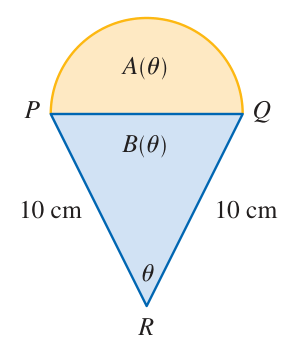
\includegraphics[height=3.15cm, keepaspectratio]{images/p0234_fig1.png}
    \vspace{-2pt}
  \end{center}

  \noindent\textbf{67.} Hình vẽ cho thấy một cung tròn có độ dài $s$ và một dây cung có độ dài $d$, cả hai đều chắn một góc ở tâm $\theta$. Hãy tìm
  \[
  \lim_{\theta \to 0^+} \frac{s}{d}
  \]
  \begin{center}
    \vspace{-5pt}
    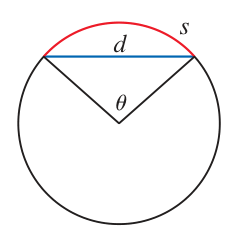
\includegraphics[height=2.25cm, keepaspectratio]{images/p0234_fig2.png}
    \vspace{-2pt}
  \end{center}

  \noindent\llap{\casicon\hspace{5pt}}\textbf{68.} Cho $f(x) = \dfrac{x}{\sqrt{1 - \cos 2x}}$.\\[3pt]
  (a) Vẽ đồ thị $f$. Hàm số dường như có loại điểm gián đoạn nào tại $0$? \enspace
  (b) Tính các giới hạn trái và phải của $f$ tại $0$. Các giá trị này có khẳng định câu trả lời của bạn ở phần (a) không?
\end{minipage}

\vspace{24pt}

% =========================================================================
% BẮT ĐẦU MỤC 3.4: QUY TẮC CHUỖI (THE CHAIN RULE)
% =========================================================================
\noindent
\begin{minipage}[c]{0.23\textwidth}
  \begin{tikzpicture}[x=1pt, y=1pt]
    \foreach \y in {-5.5, -1.8, 1.8, 5.5} {
      \draw[stewartcyan, line width=1.1pt] (0, \y) -- (\linewidth, \y);
    }
  \end{tikzpicture}
\end{minipage}%
\hspace{0.04\textwidth}%
\begin{minipage}[c]{0.73\textwidth}
  {\fontsize{22pt}{26pt}\selectfont\textsf{\textbf{\color{stewartcyan}3.4}}\quad\textsf{\textbf{Quy tắc chuỗi}}}
\end{minipage}

\vspace{10pt}

\noindent
\begin{minipage}[t]{0.23\textwidth}
  \vspace{0pt}
  \vspace{62pt} % Dóng hàng chuẩn xác với đoạn "Nhận thấy rằng F là một hàm hợp..."
  {\fontsize{8.5pt}{11pt}\selectfont\noindent\textsf{Xem Mục 1.3 để ôn lại\\về hàm hợp.}}
\end{minipage}%
\hspace{0.04\textwidth}%
\begin{minipage}[t]{0.73\textwidth}
  \vspace{0pt}
  Giả sử bạn được yêu cầu lấy đạo hàm của hàm số
  \[
  F(x) = \sqrt{x^2 + 1}
  \]
  Các công thức đạo hàm bạn đã học trong các mục trước của chương này không cho phép bạn tính $F'(x)$.

  \vspace{6pt}
  Nhận thấy rằng $F$ là một hàm hợp. Thật vậy, nếu ta đặt $y = f(u) = \sqrt{u}$ và đặt $u = g(x) = x^2 + 1$, thì ta có thể viết $y = F(x) = f(g(x))$, nghĩa là $F = f \circ g$. Chúng ta đã biết cách lấy đạo hàm của cả $f$ và $g$, vì vậy sẽ rất hữu ích nếu có một quy tắc cho biết cách tìm đạo hàm của $F = f \circ g$ theo các đạo hàm của $f$ và $g$.
\end{minipage}

\vfill
\begin{center}
{\fontsize{6.5pt}{8pt}\selectfont\color{stewartgray}
Copyright 2021 Cengage Learning. All Rights Reserved. May not be copied, scanned, or duplicated, in whole or in part. WCN 02-200-203\\
Editorial review has deemed that any suppressed content does not materially affect the overall learning experience. Cengage Learning reserves the right to remove additional content at any time if subsequent rights restrictions require it.
}
\end{center}
